\section{Progettazione concettuale}
\subsection{Analisi dei requisiti}
% \raggedright
La base dati si deve occupare della gestione del personale di un'azienda.

La figura centrale di tutto lo schema è l'impiegato.\sskip
La prima classificazione di un generico impiegato viene fatta tra:
\begin{itemize}
	\item impiegato assunto regolarmente
	\item impiegato assunto esclusivamente per lavorare ad un progetto
\end{itemize}\medskip
Gli impiegati che vengono assunti a tempo indeterminato vengono assunti con un determinato ruolo e stipendio, inoltre gli impiegati assunti regolarmente hanno diverse specializzazioni in base sia al merito sia agli anni trascorsi all'interno dell'azienda.

Dal momento in cui viene assunto, l'impiegato diventa automaticamente un junior. Trascorsi 3 anni diventa middle, passati altri 4 diventa senior.
Inoltre, qualunque siano gli anni trascorsi all'interno dell'azienda, può essere promosso e diventare manager.

Si tiene traccia di tutti gli scatti di carriera all'interno dell'entità \textit{career\_log} dove sono memorizzati:
\begin{itemize}
	\item ruolo precedente
	\item ruolo successivo
	\item data dello scatto
\end{itemize}\medskip
L'azienda è divisa in varie sedi, ogni sede ha un nome e un indirizzo.

In una sede sono presenti diversi laboratori, ognuno dei quali ha un nome e un topic di cui si occupa.\sskip
Ogni impiegato afferisce ad un unico laboratorio.\\
Un impiegato può aver anche lavorato in più laboratori ma in periodi diversi.\\
Al momento dell'assunzione l'impiegato non ha ancora una collocazione ma viene stabilito successivamente.\\
Ad un impiegato senior può essere assegnata la gestione di un laboratori o/e di un progetti.\sskip
Ad ogni laboratorio è assegnato uno scientific manager che è un impiegato senior.\sskip
L'amministratore a cui è affidata la gestione del database si occupa di:
\begin{itemize}
	\item inserire gli impiegati assunti
	\item monitorare gli scatti di carriera
	\item promuovere gli impiegati meritevoli a manager
	\item creare progetti e affidare la supervisione ad un manager e la gestione ad uno scientific referent
\end{itemize}
Per ogni progetto viene stabilita una data di partenza, una data prevista per la conclusione del progetto \textit{deadline} e dei fondi.
Può accadere che il progetto si protragga per un tempo superiore a quello previsto dalla deadline, quindi si prevede un campo \textit{end\_date} che tiene traccia dell'effettiva data in cui il progetto è terminato.

Ad un progetto possono prendere parte massimo 3 laboratori contemporaneamente, il che vuol dire che un laboratorio può decidere autonomamente quando partecipare/abbandonare un progetto.
Ogni impiegato che afferisce ad un laboratorio prende automaticamente parte a tutti i progetti a cui quel laboratorio sta lavorando

Il manager scientifico di un laboratorio decide a quali progetti partecipare e richiedere attrezzatura. Le richieste vengono memorizzate nell'entità \textit{equipment\_request}.

Le richieste vengono valutate dal manager e dallo scientific referent del progetto a cui sono state fatte, i quali decidono in base ai fondi del progetto se soddisfare le richieste, con il vincolo che il costo totale delle attrezzature non può superare il 50\% dei fondi del progetto.

Quando viene acquistata dell'attrezzatura, si salva l'acquisto nell'entità \textit{purchase} che tiene traccia della data e del prezzo d'acquisto.

Ogni attrezzatura di ogni laboratorio viene memorizzata nell'entità \textit{equipment}.\\
Un laboratorio può possedere già dell'attrezzatura e riceverne altra tramite richieste a progetti.

L'attrezzatura acquistata in un laboratorio, rimane anche dopo la fine del progetto.\sskip
Con il restante 50\% dei fondi, il manager e lo scientific referent di un progetto possono assumere del personale che viene pagato per lavorare esclusivamente per quel progetto, e non viene considerato come impiegato regolare.
Lo stesso impiegato può essere assunto più volte (anche per lo stesso progetto ma in date differenti), per questo motivo ognuno di questi impiegati viene memorizzato in maniera persistente.
La relazione \textit{works\_on} tiene traccia di tutte le volte in cui un impiegato è stato assunto per lavorare ai progetti.


\subsection{Schema concettuale}\bigskip
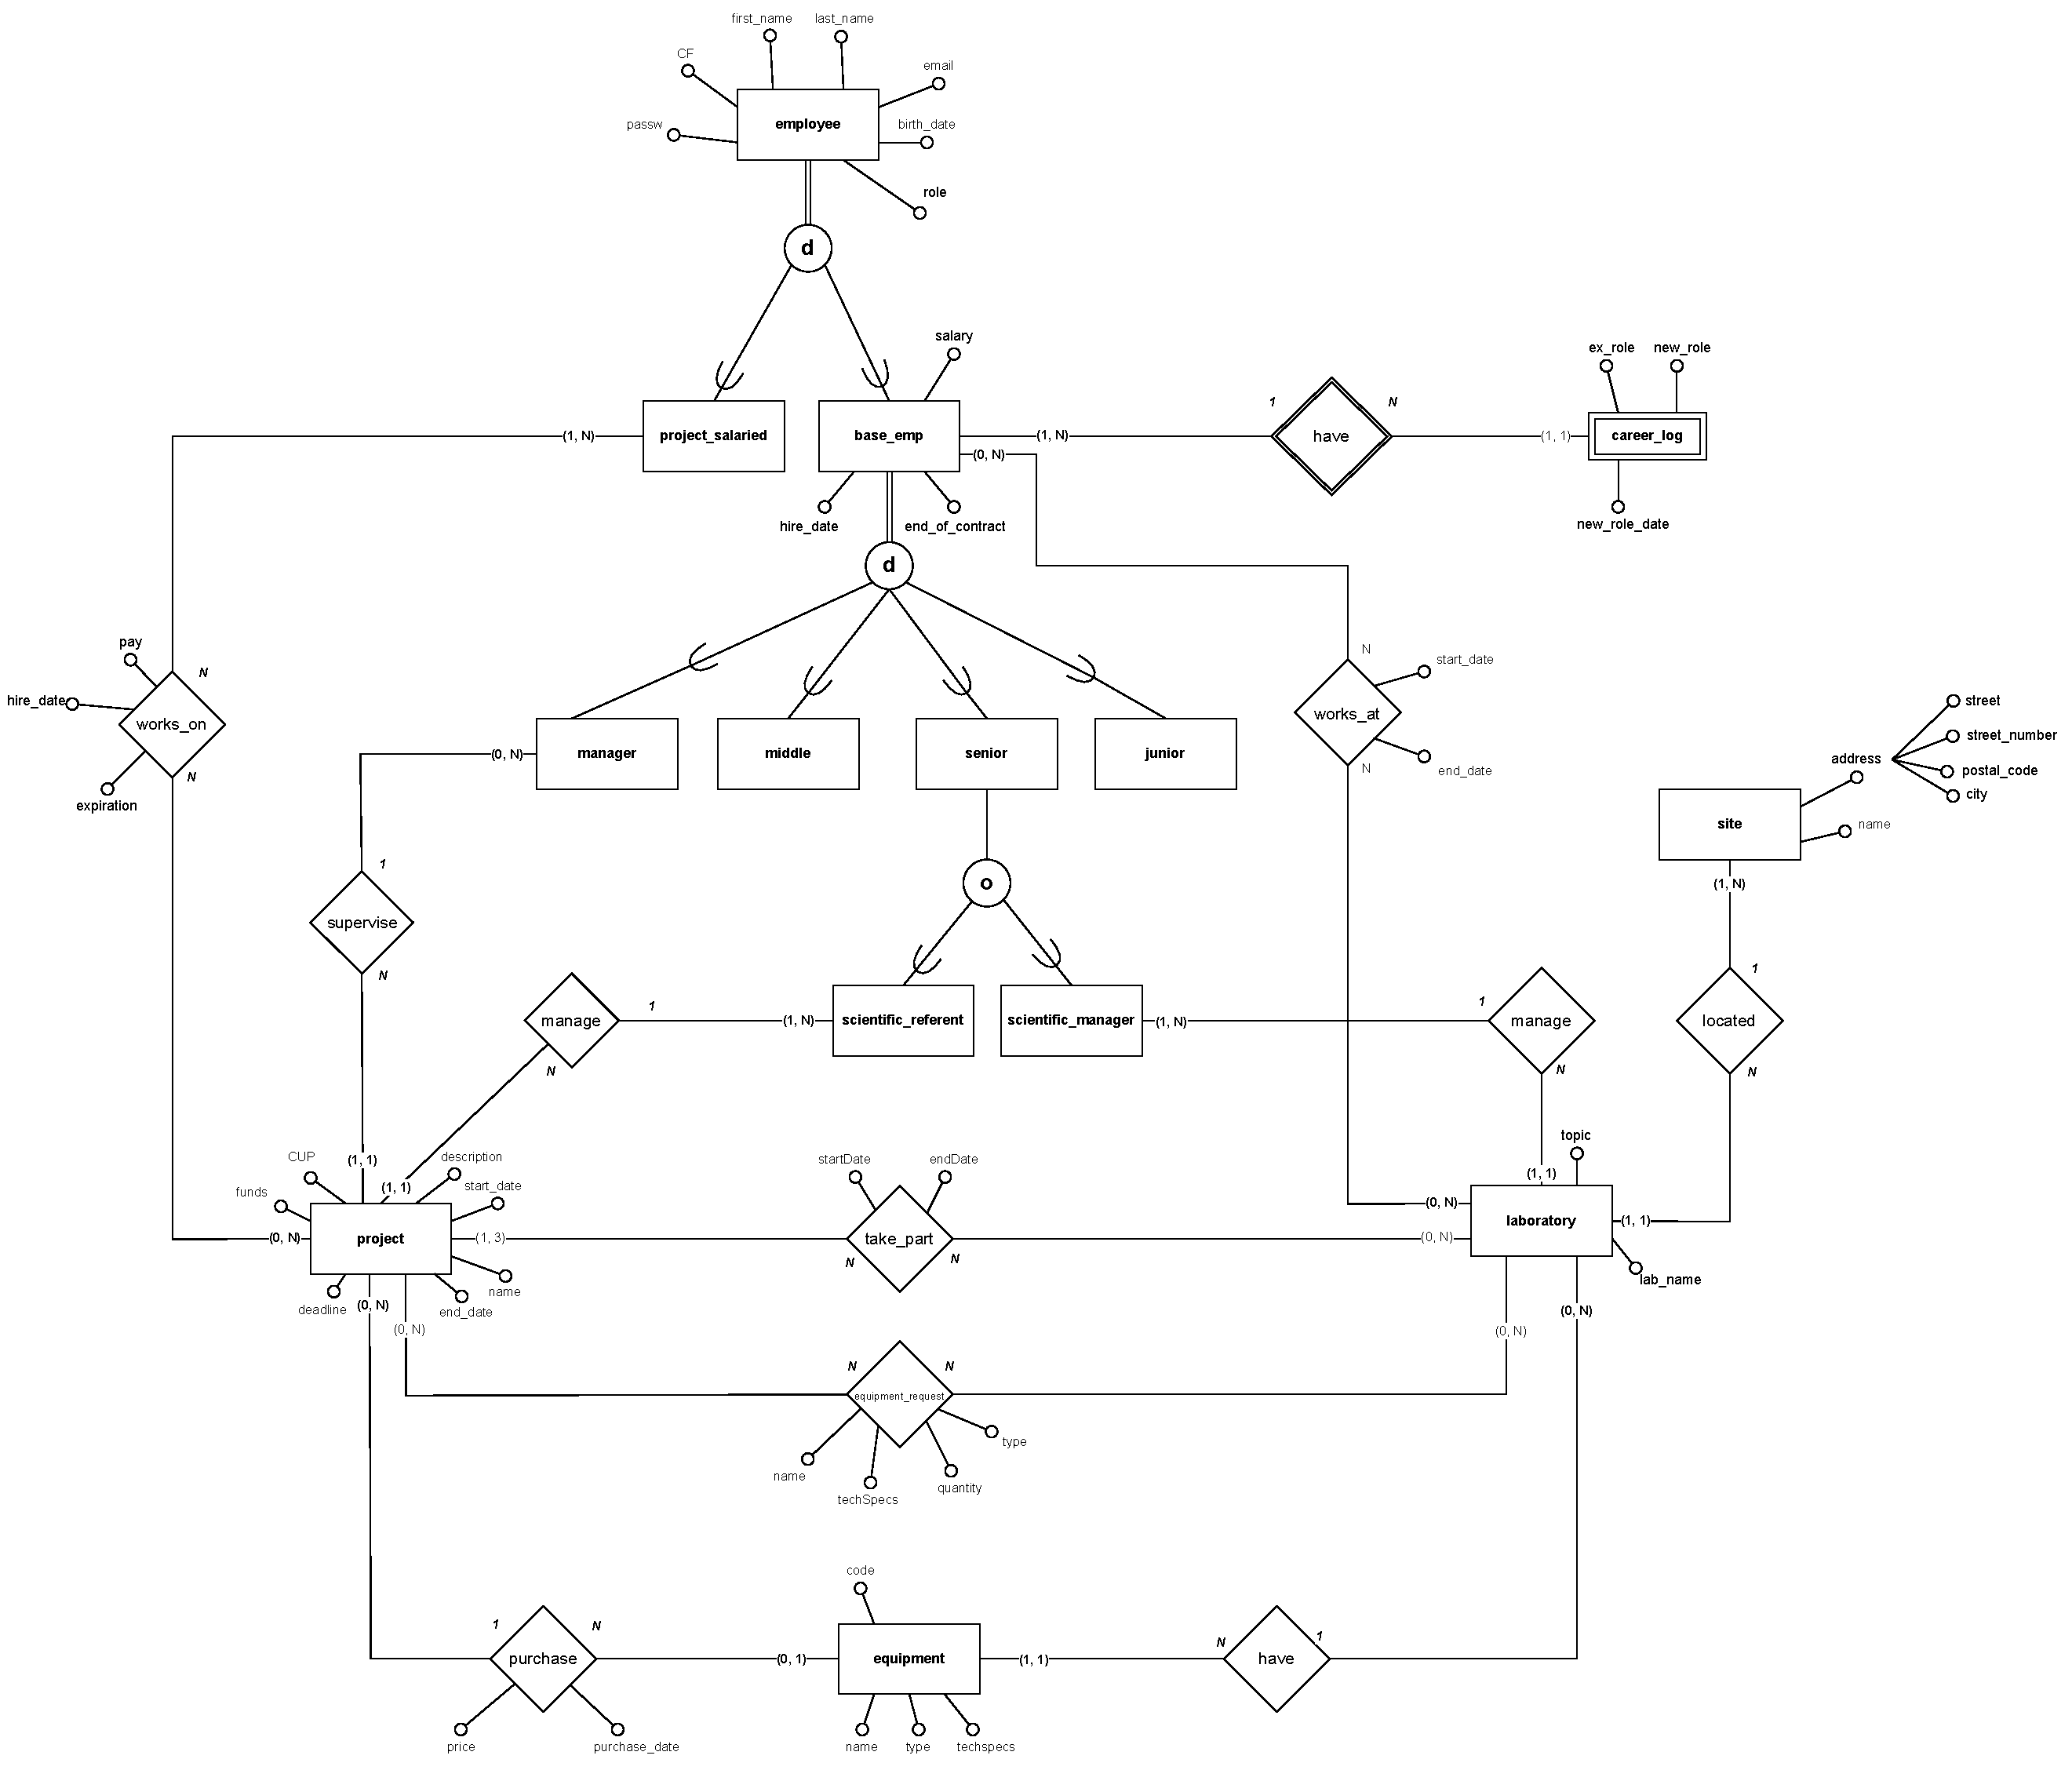
\includegraphics[width=\textwidth]{images/concettualeER.drawio.pdf}

\newpage
\subsection{Dizionario delle entità e delle associazioni}
\begin{tabular}{@{}| l | l | l |}
	\hline
	Entità & Descrizione & Attributi \\
	\hline
	col1   & col2        & col3      \\
	\hline
\end{tabular}
